\chapter{Instance segmentation}%
\label{chap:05}

\paragraph{Summary}
In this Chapter we discuss different techniques to segment different instances
of the same class in an image. To that end, we introduce the notion of bottom-up
and top-down methods which are then both discuss an more detail.

\section{Fundamentals}
We previously discussed semantic segmentation, where we want to assign a class
to each pixel in an image. If our image contains a group of people then the
semantic segmentation network might be able to find this group of people but it
is unable to decide where one person ends and where the next person begins.
This is precisely the goal of instance segmentation: we want to find all
individual instances of a particular class. More precisely, we will call this
task semantic instance segmentation or panoptic segmentation (since we try to
identify different classes and within each class identify the individual
instances). If there is only one class present, then we will refer to the task
of identifying the individual instances of this single class as instance
segmentation without segmentation or image partitioning; one example is
illustrated in the Figure below.
\begin{figure}[htpb]
  \centering
  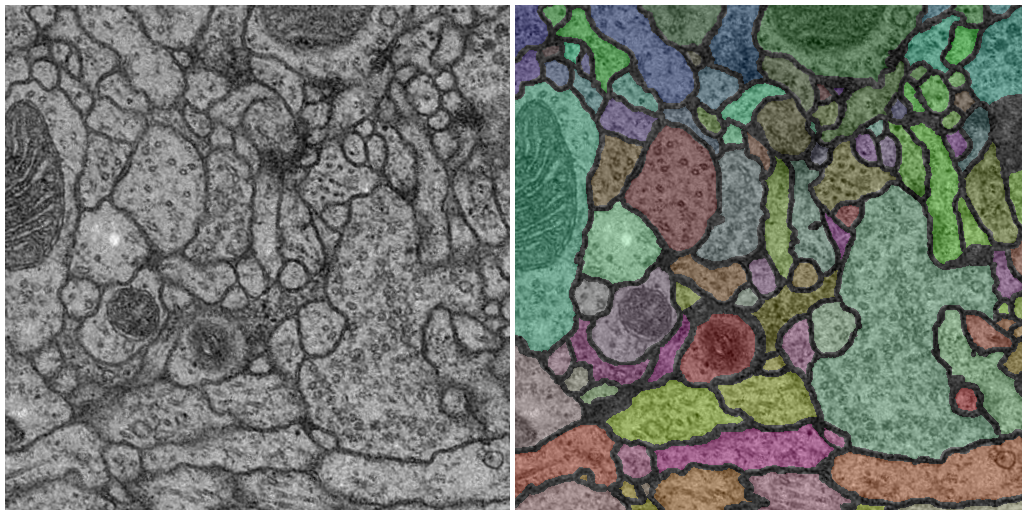
\includegraphics[width=0.7\textwidth]{Figures/instance_segmentation}
  \caption{Example of an image of neural structures in a brain and the
    corresponding instance segmentation.}%
  \label{fig:instanceseg}
\end{figure}
Note that the colours in the partitioned image are chosen randomly and are not
important; what is important is that two pixels that have the same colour belong
to the same instance. Another example where a little bit of semantics have to be
learned is instance segmentation with the additional task of deciding whether a
pixel is background or foreground. The instance segmentation is then done only
for the foreground pixels; the background that has only to be identified as
such. What all of these problems have in common is that the number of instance
that we try to identify is not known beforehand. If we know that there will be a
fixed number of instances in the image, different methods should be used that we
will not discuss in this lecture.

The general strategies to solve these kinds of problems can be broadly
categorised into \emph{top-down} and \emph{bottom-up} approaches.
\begin{itemize}
\item Top-down\qquad This approach is also called \emph{proposal-based}. Here,
  we first try to find one seed (\ie, the centre of the instance) or one
  bounding box for each instance and only then try to estimate the precise shape
  of that instance. One approach to find the exact shape given a bounding box
  would be to divide the bounding box into, for example, $16 \times 16$ pixels
  and classify each pixel (does it belong to the instance or not) using
  techniques discussed earlier.
\item Bottom-up\qquad This \emph{proposal-free} strategy can be again divided
  into two sub-strategies. The first can be seen as a generalised Hough
  transform (discussed below) where each pixel directly votes for instance
  membership. This then implicitly also gives the shape of the particular
  instance. In the second approach we try to decide for pairs of pixels whether
  or not they belong to the same instance and we were to do this for all of the
  pixels and all possible pairs this would give as a signed graph. This signed
  graph can then be partitioned in the ``least hurtful'' way.
\end{itemize}

\section{Proposal-based methods}
There is a wide variety of top-down strategies that have successfully been used
in the past. The following generic algorithm tries to summarise the general
underlying idea which in essence can be interpreted as a sliding window
approach.
\begin{enumerate}
\item For each location answer one or more of the following questions.
  \begin{itemize}
  \item Am I a seed?\hfill {\color{gray}Classification}
  \item If I am a seed, to what class do I belong? \hfill
    {\color{gray}Classification}
  \item Relative to me, where is the closest seed? \hfill
    {\color{gray}Regression}
  \item What is the bounding box relative to my location? \hfill
    {\color{gray}Regression}
  \end{itemize}
\item Usually, the first step will produce several seeds or several bounding
  boxes for each instance but of course we only want one seed or one bounding
  box. Therefore, we have to somehow decimate them. We call this step the
  inference step; it is discussed in more detail below.
\item Having now only one seed or one bounding box, we can estimate precises
  mask or outline of the respective instance conditioned on the surviving seeds
  from the previous step.
\end{enumerate}
A simple technique for improving the first step is to slide windows of several
aspect ratios and sizes across the image simultaneously (instead of just a
single window) and asking these questions for every size.

Below we will discuss some strategies that can be used in the inference step. As
mentioned above, we will likely have multiple bounding boxes or multiple seeds
that where there should only be one. The following is a very simple method to
``clean up'' the additional, unwanted seeds and boxes. There are more advanced
variants of this algorithm and also other methods to solve this problem.

\subsection*{Non-maximum suppression}
After the first step in the generic algorithm above, we have possibly multiple
detections for each instance. To each of these detection a probability is
assigned and we start by taking the overall detection with the largest
probability and set it to be the first actual detection. When the ``kill'' every
detection in a fixed neighbourhood of this detection. Thereafter, we do the same
thing again but with the second most plausible detection. Since we removed all
the detections in the vicinity of our first true detection, we hope that the
second largest detection belongs to a different instance in the image. This is
repeated until no detections are left. We do also apply a threshold and
detections below that threshold will not be considered (they are considered as
being too unlikely).

\section{Hough Transform}
In general, Hough transform is a feature extraction technique; more precisely it
can be used to find imperfect instances of parameterised objects by a voting
procedure. This voting procedure is carried out in a parameter space, from which
object candidates are obtained as local maxima in a so-called accumulator space.

In the simplest case of the Hough transform, the goal is to detect straight
lines. Since the ``classic'' parametrisation $y = mx + b$ leads to unbounded
values in the case of vertical lines, one rather uses the form
$r = x \cos \theta + y \sin \theta$, where $r$ is the distance from the origin
to the closest point of the straight line, and $\theta$ is the angle between the
$x$ axis and the line connecting the origin with that closest point (of course
other parametrisations are also possible). It is now possible to assign to each
line a pair $(r,\theta)$, or a point in the $(r,\theta)$ plane.

Given a single point in the plane, the set of all straight lines going through
that point corresponds to a sinusoidal curve in the $(r,\theta)$ plane and this
curve is unique to this point. A set of two or more points that form a straight
line will produce sinusoids which cross at the $(r,\theta)$ point that
parameterises this line.

\section{Similarity Learning}
Instead of directly learning whether or not to pixels are similar we learn a
mapping $e$ from the observations (\ie, the image) $X$ into some embedding space
$\mathbb{E}$ (\eg, $\R^k$). We can then compute the similarity of two pixels
$x_1$ and $x_2$ by computing their respective distance in the embedding space,
\ie we compute
\begin{equation*}
  s(x_1,x_2) = s_{\mathbb{E}}(e(x_1),e(x_2)) = s_{\mathbb{E}}(e_1,e_2)\,.
\end{equation*}
This is usually more efficient, since the distance in the metric space is
typically simpler to compute (for example, $s_{\mathbb{E}}$ might just be the
Euclidean distance). The loss function to train the neural network which in this
case is called contrastive loss or associative loss is given by the following
equation
\begin{equation*}
  L = \sum_{x_i,x_j} \delta_{c_i\,c_j}(1 - s(e(x_i), e(x_j))) + (1 - \delta_{c_i\,c_j}){[s(e(x_i),e(x_j)) - \alpha]}_+\,,
\end{equation*}
where $c_i$ and $c_j$ are the associated instance of pixel $x_i$ and pixel
$x_j$, respectively. Thus, the first part inside the sum is ``turned on'' if two
pixels belong to the same instance whereas the second part is turned on when
they belong to different instances. Since in the former case we would like the
loss to be low, \ie their similarity should be high. In the latter case we want
their similarity to be low (here ${[x]}_+ = \max(0,x)$, \ie similarities below a
threshold of $\alpha$ will be cut off).


%%% Local Variables:
%%% mode: latex
%%% TeX-master: "../main"
%%% End:
